% !TEX root = DesignDocument.tex


\chapter{Overview and concept of operations}

%The overview should take the form of an executive summary.  Give the reader a feel 
%for the purpose of the document, what is contained in the document, and an idea 
%of the purpose for the system or product. 

\section{Bowtaps and its team}

Bowtaps is a start up company out of SDSM\&T created by the team members of Bowtaps. Our goal is to create easy to use software applications that help ease the everyday life of the user. Bowtaps currently consists of the members Charles Bonn, Johnathan Ackerman, Daniel Andrus, Evan Hammer, and Joesph Mowry.

\section{Crowd Control}
Our flag-ship product(Crowd Control) is to create a mobile application that combines GPS tracking, group messaging and group management features into one easy to use application. 

\subsection{Purpose of the System}
Crowd Control is a mobile application designed to ease the experience of going out though the implementation of integrated group messaging, GPS tracking and group management features. Along with the features to manage your group at the event Crowd Control also gives suggestions of local events, restaurants and attraction. This allows the group to continue even when the next item on the agenda is a mystery. 


Even though Crowd Control is designed for the party scene, and people going out to events; it's uses can be expanded to fit more purposes. Crowd Control can be used to help manage any kind of group at an event such as church groups, tour groups, or school field trips.

\section{Business Need}
\begin{comment}
Use this section to define what business need exist and how this software will 
meet and/or exceed that business need.   (still fill out)
\end{comment}

(TODO)

\section{Deliverables}
\begin{comment}
Provide a complete description of the client requested deliverables.   This section should be the section your software contract references.   ( still fill out)
\end{comment}
(TODO)

\section{System Description}
Behind the UI, Crowd Control is written using an MVC architecture. IOS is written natively in Swift under the IDE XCode. On the Android side, the code is written in Native Mobile Java under Android Studio.

The code for Android uses xml files for layouts which act as the view in MVC. Each activity acts as a controller. Each one of the models has an interface, which is how the controllers get access to the functions and data provided by the model. Each interface is set up in such a way that it uses OOP inheritance to generalize the models, thus abstracting our third party software.\\

(TODO) IOS??

\subsection{Integrated Group Messaging}
Integrated group messaging is an important feature of Crowd Control. It allows for communication between cross platform, different phone brands, and different carriers. This allows for seamless communication between users with out the issues associated with messaging such as messages not using the same format, messages not going to all recipients, and messages with users in the group that you do not want to have your personal information.

Currently this is handled by a third party called Sinch. Sinch messaging handles the encryption of messages for the security of our users. Also, Sinch uses app to app messaging. In this way, any device with Crowd Control can send a message to other group members. However, since our app is currently only implemented on Android, messages can only be passed between Android users. It only needs either an internet connection or cell service to function.

\subsection{GPS Location services}
GPS allows for tracking of members in the group on a local map of the area. With this feature you will be able to keep track of anyone in the group off of their last GPS check in. This is useful to help locate members of the group that maybe lost or unable to be located. This feature will have the option of being able to opt out when the user does not want to have their location known to the group. When the users battery is low it will allow for the check in period to be extended or turned off to save battery life.

(TODO)

\subsection{Group Management Features}
The group management features allow for information to be shared with the group. A group management menu will allow for a group agenda to be posted as well as updates when the agenda changes. With the GPS features it will allow for the group leader to set way-points for the group.  

\subsection{Suggestions}
Suggestions are both a plus for the user and our way of making revenue. Suggestions are sponsored by local businesses in the form of an ad. Although these are not traditional ads, they are in the form of local points of interest such as restaurants, bars, amusement parks, or bowling allies. The possibilities are endless. With the suggestion method it will allow for our users to have helpful suggestions of places for their group to attend as well as exposure for the local businesses that are sponsoring Crowd Control.


\section{System Overview and Diagram}
The basic overview of Crowd Control can be seen in the diagram below. See Figure~\ref{ModuleFlowDiagram}. Crowd Control will be using a model-view-controller design structure. With the model view controller design method we are able to abstract the user interface from the control structures that will communicate with the third party services such as Parse, Google play services, or Sinch. The model of each respective operating system ( Android or iOS ) will be able to communicate with the respective mapping feature ( Google Play Services or Apple Map Features ). While both models will be able to communicate with Parse, our back end server. Though Parse, using their features, will be able to connect user profiles to their Facebook and twitter accounts for faster log in.

\begin{figure}[tbh]
\begin{center}
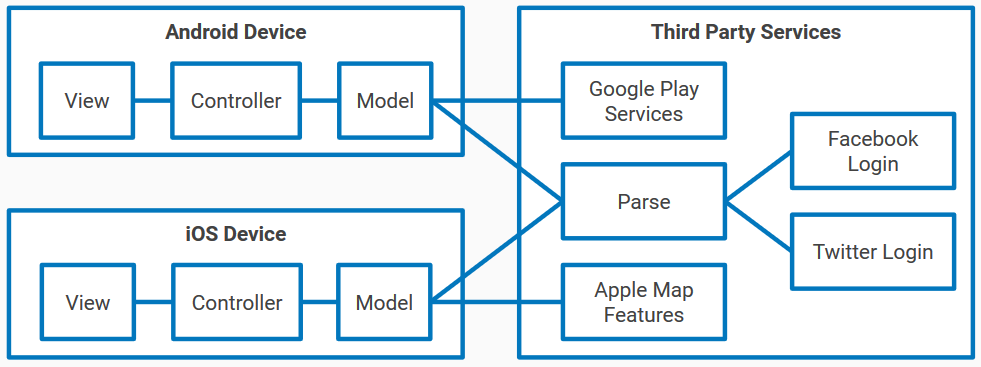
\includegraphics[width=0.75\textwidth]{Additional/designpictures/ModuleFlowDiagram.png}
\end{center}
\caption{Basic System Flow Diagram \label{ModuleFlowDiagram}}
\end{figure}

\section{Technologies Overview}
Some technologies used in the creation of Crowd Control are Google Play Services, Apple Map Features, Parse, Sinch, and Android Studio.

\subsection{Google Play Services}
	\subsubsection{Description}
	Google Play Services contains the native android API for mapping features. With this it allows for communication between a map and your GPS location along with other mapping features.
\newline
REFERENCE LINK:  \url{https://developers.google.com/android/guides/setup}
	\subsubsection{Usage}
	Google Play Services will be used on the Android device as the default map. We chose to go with Google Play services to give android users a more native feel when it comes to using the mapping features. This allows for a less intrusive feel when it comes to using Crowd Control, will be used for displaying your location on a map, displaying other users in your group on a map, and displaying event suggestions on the map.

\subsection{Apple Map Features}
	\subsubsection{Description}
	Apple Map Features is the native iOS API for mapping features. With this it allows for commiseration between a map and your gps location along with other mapping features.
\newline
REFERENCE LINK: \url{https://developer.apple.com/maps/}
	\subsubsection{Usage}
	Apple Map Features will be used on the iOS device as default. We chose to go with Apple Map Features to give iOS users a more native, less intrusive feel. This will be used for displaying your location, displaying other users from your group, and displaying local event suggestions on the map.

\subsection{Parse}
	\subsubsection{Description}
	Parse is abstracted behind all of our models. Our usage of it is restricted to the functions we provided ourselves though the implementations of our models, keeping all of the actual parse code out of the controllers. Parse gives us access to a web-based database that is fully protected by an experienced third party.
\newline
REFERENCE LINK: \url{http://parse.com/}
	\subsubsection{Usage}
	Parse is abstracted behind all of our models. Our usage of it is restricted to the functions we provided ourselves though the implementations of our models, keeping all of the actual parse code out of the controllers.
	Parse is our back-end database. It saves all the group information into a web accessible parse database, as well as storing personal log in information to another Parse database local to the phone. The globally stored information is paced among members of the group, were as the locally stored information is used for automatic log in at the convenience of our users. The web-based storage will also hold all of the location values(though encrypted), and by using a service, will keep those value up-to-date on any given device.
	
\subsection{Sinch}
	\subsubsection{Description}
	Sinch is a third party, device to device, communication API. We have selected it for its encryption, and ready to use app-to-app messaging platform. This platform will work with either wi-fi connection, or cell service. 
\newline
REFERENCE LINK: \url{https://www.sinch.com/}
	
	\subsubsection{Usage}
	Sinch has its own service to handle the sending and receiving of messages. We have constructed a fragment(with the help of some Sinch code) to control a user interface to grab messages passed by the user. We have also modified the basic one-to-one message sending to send the message to the entire group.



